% LegacyCRM-Bench — OJ-CS submission draft.
% STATUS: DRAFT — NOT SUBMISSION-READY. See 10_submission_package/SUBMISSION_READINESS_REPORT.md.
% This draft uses the IEEEtran class as a stand-in. Before submission it MUST be ported to the
% official IEEE Open Journals template downloaded from https://template-selector.ieee.org/
% (blocker E9 in 04_experiments/EVIDENCE_REQUIRED.md). Do not alter margins/type sizes/spacing.
% Headline quantitative values are injected from generated/numbers.tex (produced by
% analysis/make_tex_tables.py from raw results); prose range summaries are transcribed from
% the released M1-M5 tables and were independently re-derived in the cycle-2 audit.
\documentclass[journal]{IEEEtran}
\usepackage{booktabs}
\usepackage{graphicx}
\usepackage{url}
\usepackage[hidelinks]{hyperref}
% auto-generated by make_tex_tables.py — do not edit
\newcommand{\NumCases}{36}
\newcommand{\NumTests}{521}
\newcommand{\NumEasy}{12}
\newcommand{\NumMedium}{12}
\newcommand{\NumHard}{12}
\newcommand{\RefPassed}{521}
\newcommand{\RefTotal}{521}
\newcommand{\NullPassed}{0}
\newcommand{\NumMutants}{363}
\newcommand{\MutantsKilled}{352}
\newcommand{\KillRate}{97.0}
\newcommand{\SurvivingMutants}{11}
\newcommand{\SeedRows}{716}
\newcommand{\KillRateCILo}{94.7}
\newcommand{\KillRateCIHi}{98.3}
\newcommand{\PTwoGens}{1980}
\newcommand{\PTwoFails}{31}
\newcommand{\RepairCalls}{11}
\newcommand{\RepairUnfixed}{0}
\newcommand{\SpendTotal}{33.59}


% ------- DRAFT watermark (remove only when readiness criteria are met) -------
\usepackage{atbegshi,tikz}
\AtBeginShipout{\AtBeginShipoutUpperLeft{%
  
\begin{tikzpicture}[remember picture,overlay]
    \node[rotate=55,scale=7,text opacity=0.12] at (current page.center)
      {DRAFT -- NOT FOR SUBMISSION};
  \end{tikzpicture}}}

\begin{document}

\title{LegacyCRM-Bench: A Reproducible Benchmark for Evaluating LLM-Assisted Migration of
Enterprise CRM Customizations\\
{\normalsize [DRAFT v0.3, 2026-09-02 --- full frozen-protocol evaluation executed;
DRAFT status reflects open administrative blockers only]}}

\author{Chitrapradha~Ganesan,~\IEEEmembership{Senior~Member,~IEEE}%
\thanks{The author is with the Post Graduate Program in Artificial Intelligence and Machine
Learning, The University of Texas at Austin, Austin, TX 78712 USA (e-mail:
chitracrmexpert@gmail.com).}%
\thanks{Corresponding author: Chitrapradha Ganesan (e-mail: chitracrmexpert@gmail.com;
ORCID: 0009-0009-1305-1724).}}

\maketitle

\begin{abstract}
Enterprises modernizing legacy customer relationship management systems must migrate a
customization layer: validation rules, workflow automations, scripts, access-control
matrices, integrations, and audit behavior. Large language models are increasingly proposed
to assist this work, yet existing benchmarks evaluate agents operating inside a fixed system
or translation of function-level code; to our knowledge none measures whether a migration
preserves the behavior of configured enterprise customizations. We present LegacyCRM-Bench,
built on a fictional legacy system whose complete semantics the benchmark specifies and
owns: \NumCases{} migration cases across twelve categories with \NumTests{} executable
acceptance tests covering functional, security, privacy, and audit preservation. The
instrument is validated end to end: reference solutions pass every test, an empty-solution
control passes none, and mutation-guided strengthening reaches a \KillRate\% kill rate with
every surviving mutant classified. A deterministic transpiler solves eleven cases outright,
and \PTwoGens{} sandboxed generations then evaluate three commercial models under
zero-shot, guided-prompting, and repair conditions. Case-level scores are near ceiling, yet repeated-trial
reliability separates the model tiers, remaining failures concentrate on
legacy-convention, cross-artifact, schema-completeness, and access-control-equivalence
oracles, a structured
checklist prompt is accompanied by reproducible access-narrowing regressions that zero-shot
prompting avoids, and redacted-feedback repair fixes every observed failure. All artifacts are prepared for public release.
\end{abstract}

\begin{IEEEkeywords}
Benchmarking, software migration, legacy modernization, large language models, access control.
\end{IEEEkeywords}

\section{Introduction}
\label{sec:intro}
% [Verified context: verified references; no unverified market figures are cited.]
Customer relationship management platforms accumulate customizations over years of operation:
declarative validation rules, workflow state machines, procedural scripts, role-based
access-control (RBAC) matrices, integration endpoint configurations, batch jobs, and audit
policies. When an organization replatforms, this layer is where semantics must be re-derived
and re-implemented, because they are often implicit, idiosyncratic, and enforced by convention
(sentinel values, soft-delete flags, evaluation order) rather than by types or schemas. LLM assistance is an
attractive proposition for such migrations, but the field currently lacks a way to measure
\emph{behavioral preservation} of the customization layer under migration, including its
security semantics.

Benchmarks exist on either side of this gap. The CRMArena line~\cite{huang2025crmarena,
huang2025crmarenapro} measures whether agents can operate a realistic CRM; enterprise sandboxes
such as EnterpriseBench~\cite{vishwakarma2025enterprisebench}, WorkBench~\cite{styles2024workbench},
WorkArena~\cite{drouin2024workarena}, and $\tau$-bench~\cite{yao2024taubench} measure task
completion inside fixed environments, some with access-control awareness. Code-translation
research measures execution equivalence at function or repository
granularity~\cite{lachaux2020transcoder, yan2023codetransocean, pan2024lost,
ibrahimzada2025alphatrans}, and industrial COBOL-modernization pipelines validate translated
programs against generated tests~\cite{hans2025coboltesting, kumar2025cobolvalidation,
froimovich2025cobolquality}. To our knowledge, none of these evaluates whether a migration of \emph{configured
platform behavior} (rules, workflows, permissions, audit) preserves that behavior.

LegacyCRM-Bench fills this gap with three design commitments. First, the legacy system is
\emph{synthetic and fully documented}: a fictional product, ``Meridian CRM 4.2,'' whose SQL
schema, validation-rule domain-specific language (DSL), workflow XML, scripting language,
RBAC matrix, and configuration
formats are specified in a frozen semantics document authored with the benchmark. This makes
ground truth hand-derivable, eliminates proprietary-data risk, and gives a contamination
argument by construction for the artifacts themselves. Second, every case carries
\emph{executable preservation oracles}: pytest acceptance tests whose expected values are
derived in writing from the documented semantics, including negative expectations (behavior
that must be rejected), security expectations (no privilege widening, no credential literals,
privacy exclusions), and hallucination checks (no invented states, codes, or permissions).
Third, the harness is \emph{deterministic and offline}, so every reported number is
reproducible from the released artifact.

This paper reports the benchmark's construction, its instrument validation (reference,
null-baseline, and mutation evidence), and a complete execution of the frozen evaluation
protocol: a deterministic-transpiler control plus three commercial models under four
conditions with five repeated runs per cell, all inside a network-denied sandbox with the
oracle unreachable at runtime. Every reported number is machine-generated from the released
raw logs.

\section{Related Work}
\label{sec:related}
\subsection{CRM and Enterprise Agent Benchmarks}
CRMArena~\cite{huang2025crmarena} and CRMArena-Pro~\cite{huang2025crmarenapro} are established
CRM benchmarks: synthetic but expert-validated Salesforce-style organizations in which agents
perform professional tasks, with CRMArena-Pro adding multi-turn interaction and
confidentiality-awareness probes. EnterpriseBench~\cite{vishwakarma2025enterprisebench}
simulates a fragmented enterprise with access-control hierarchies; WorkBench~\cite{styles2024workbench}
uses outcome-centric evaluation over sandboxed workplace databases including CRM-like data;
WorkArena~\cite{drouin2024workarena} evaluates web agents on a live ServiceNow instance;
AgentBench~\cite{liu2023agentbench} and AgentBoard~\cite{ma2024agentboard} evaluate general
agent ability. $\tau$-bench~\cite{yao2024taubench} contributes database-state-diff evaluation
and the pass\textasciicircum{}$k$ reliability metric, which our protocol adopts. All of these
evaluate agents \emph{operating} a fixed environment; none evaluates transformation of the
environment's customization layer. LegacyCRM-Bench is therefore not the first CRM benchmark and
does not claim to be; its object of evaluation is different.

\subsection{Code Translation and Migration}
TransCoder~\cite{lachaux2020transcoder} introduced execution-checked neural translation;
CodeTransOcean~\cite{yan2023codetransocean} broadened coverage to low-resource and
modernization-flavored pairs; Pan et al.~\cite{pan2024lost} taxonomized LLM translation bugs
across 1{,}700 samples; Eniser et al.~\cite{eniser2024rust} studied real-world translation to
Rust. AlphaTrans~\cite{ibrahimzada2025alphatrans} performs repository-level translation with
fragment-wise differential validation, the closest methodological relative of our oracles.
PyMigBench~\cite{islam2023pymigbench} and its LLM follow-up study~\cite{islam2025libmigration}
benchmark library-API migration. Industrial work on COBOL-to-Java
modernization~\cite{diggs2024legacy, hans2025coboltesting, kumar2025cobolvalidation,
froimovich2025cobolquality} validates translated programs, generally on artifacts that cannot
be fully released. These lines establish translation-correctness evaluation for
\emph{general-purpose code}; LegacyCRM-Bench extends the question to multi-artifact platform
customizations where correctness includes RBAC, audit, privacy, and configuration-completeness
properties, and packages it as an open benchmark.

\subsection{Code-Generation Benchmarks, Oracles, and Contamination}
HumanEval~\cite{chen2021humaneval}, MBPP~\cite{austin2021mbpp}, CodeXGLUE~\cite{lu2021codexglue},
RepoBench~\cite{liu2023repobench}, BigCodeBench~\cite{zhuo2024bigcodebench}, and
SWE-bench~\cite{jimenez2024swebench} define the execution-oracle tradition we follow.
EvalPlus~\cite{liu2023evalplus} showed that weak test suites inflate pass rates, motivating our
mutation analysis, whose lineage runs through differential testing~\cite{yang2011csmith}.
Contamination studies~\cite{golchin2024timetravel, sainz2023contamination} and
LiveCodeBench~\cite{jain2024livecodebench} motivate our synthetic-provenance design and dated
release; rigorous-agentic-benchmark guidance~\cite{zhu2025rigorous} informs our validity
checks. Security evaluation of generated code~\cite{pearce2022asleep, bhatt2023cyberseceval,
bhatt2024cyberseceval2} and access-control change-impact analysis~\cite{fisler2005margrave}
underpin our security-preservation oracles. Statistical practice follows
\cite{miller2024errorbars, efron1979bootstrap, dror2018hitchhiker}.

\section{Research Gap and Contributions}
\label{sec:gap}
The gap: to our knowledge (systematic search log in the artifact), no existing benchmark measures whether LLM-assisted migration preserves the behavior
of enterprise CRM customizations, including security semantics, under transformation from a
legacy platform to a modern target. Our contributions are:
(1)~a fully documented synthetic legacy CRM (schema, rule DSL, workflow engine, scripting
language, RBAC, integrations, batch, audit) with deterministic seed data;
(2)~\NumCases{} migration cases across twelve categories with hand-derived, executable
preservation oracles (\NumTests{} tests), including security, privacy, and hallucination
checks;
(3)~a deterministic offline harness with structural validation, null-baseline control, and
mutation-sensitivity analysis, plus machine-generated tables traceable to raw logs;
(4)~a frozen evaluation protocol (conditions, metrics, statistics, contamination controls)
with sandboxed execution; and (5)~a complete execution of that protocol --- deterministic
transpiler control plus three commercial model tiers, five runs per cell --- yielding the
calibration, reliability, and checklist-regression findings of Secs.~\ref{sec:results}
and~\ref{sec:ablation}. We explicitly do not claim novelty for CRM benchmarking per se, for
execution-based translation oracles, or for migration benchmarks in general
(Sec.~\ref{sec:related}).

\section{Research Questions}
\label{sec:rqs}
\textbf{RQ1 (Fidelity):} To what extent do LLM-assisted migrations preserve documented legacy
behavior, by test pass rate and case-level all-pass rate?
\textbf{RQ2 (Property classes):} Which preservation properties fail most often: functional
logic, ordering/rounding conventions, security semantics, privacy exclusions, audit fidelity,
or structural completeness?
\textbf{RQ3 (Condition effect):} Do structured prompting, specification retrieval, or
test-feedback repair improve preservation, at what cost?
\textbf{RQ4 (Reliability):} How consistent are outcomes across repeated runs
(pass\textasciicircum{}$k$)?
Sec.~\ref{sec:results} answers RQ1--RQ4 from the executed protocol, after first answering
the prerequisite instrument-validity question, \textbf{RQ0}: do the oracles measure what
they claim to measure?

\section{Benchmark Design Goals}
\label{sec:goals}
\textbf{G1 Preservation-centric oracles.} Correctness is defined as fidelity to documented
legacy semantics, not similarity to any reference text. \textbf{G2 Hand-derivable ground
truth.} Every expected value must be derivable from the written semantics; each case includes a
numbered derivation document. \textbf{G3 Security as first-class.} RBAC equivalence,
deny-by-default, credential hygiene, privacy exclusions, and audit fidelity are tested, not
assumed. \textbf{G4 Determinism.} No network, no wall-clock, fixed seeds, pinned dependencies.
\textbf{G5 License safety.} All artifacts synthetic and openly licensed (MIT/CC~BY~4.0).
\textbf{G6 Contamination transparency.} Artifacts are novel and dated; the release note states
that post-release training may contaminate future evaluations. \textbf{G7 Honest scale.} A
pilot of \NumCases{} rigorously validated cases is preferred over a larger, weakly validated
set; scale-up is future work.

\section{CRM Migration Task Taxonomy}
\label{sec:taxonomy}
Cases are organized into twelve categories covering common customization mechanisms found in
mainstream CRM platforms (the mechanisms we deliberately exclude from the pilot are listed in
Sec.~\ref{sec:limitations}): schema and field mapping; validation rules; business workflows;
legacy scripts; role-based access controls; integration interfaces; batch processing; error
handling; audit logging; referential integrity; business-rule preservation; and configuration
modernization. Each category contains an easy, a medium, and a hard case under a written
difficulty rubric (single-convention mapping; interacting conventions; cross-entity or
security-critical semantics where plausible migrations pass naive checks). Table~\ref{tab:comp}
gives the composition.

\begin{table}[t]
\caption{Benchmark composition (machine-generated from case metadata).}
\label{tab:comp}
\centering
\begin{tabular}{lccccc}
\toprule
Category & Cases & Easy & Med. & Hard & Tests \\
\midrule
Audit logging & 3 & 1 & 1 & 1 & 39 \\
Batch processing & 3 & 1 & 1 & 1 & 39 \\
Business rules & 3 & 1 & 1 & 1 & 42 \\
Config.\ modernization & 3 & 1 & 1 & 1 & 43 \\
Error handling & 3 & 1 & 1 & 1 & 41 \\
Integration & 3 & 1 & 1 & 1 & 43 \\
Legacy scripts & 3 & 1 & 1 & 1 & 48 \\
RBAC & 3 & 1 & 1 & 1 & 42 \\
Referential integrity & 3 & 1 & 1 & 1 & 38 \\
Schema mapping & 3 & 1 & 1 & 1 & 44 \\
Validation rules & 3 & 1 & 1 & 1 & 54 \\
Workflows & 3 & 1 & 1 & 1 & 48 \\
\midrule
\textbf{Total} & \textbf{36} & \textbf{12} & \textbf{12} & \textbf{12} & \textbf{521} \\
\bottomrule

\end{tabular}
\end{table}

\section{Dataset and Artifact Construction}
\label{sec:dataset}
\textbf{The legacy system.} Meridian CRM 4.2 is a fictional early-2000s on-premises CRM,
authored for this benchmark. Its artifacts are: a legacy-dialect SQL schema over ten entity
families (accounts, contacts, opportunities, cases, products, orders and order lines,
activities, users and roles, integration endpoints, audit events) with application-enforced
integrity; a data dictionary with status-code semantics and fixed-width export layouts; a
line-oriented validation-rule DSL (``VRL'' in the released artifact) with collect-all error
semantics and BLOCK/WARN
severities; XML workflow definitions with guards, ordered actions, first-match transition
selection, and escalation timers; a BASIC-like scripting language (CRMScript) with documented
quirks (empty-string numeric coercion, division-by-zero yielding zero with an audit event);
an RBAC matrix over roles, objects, actions, and scopes (ALL/TEAM/OWN/NONE) with
deny-by-default; INI-based integration endpoints whose credentials are vault references; a
batch schedule with ABORT/CONTINUE/RETRY error policies; and an append-only, per-column audit
configuration. The complete semantics are frozen in a specification document that, together
with the normative comments embedded in the legacy artifacts themselves, is the authority for
expected behavior. Legacy conventions that make migration hazardous, such as
sentinel dates (\texttt{00000000}), blank-means-default codes, soft-delete flags, and
denormalized totals, are used consistently across artifacts.

\textbf{Seed data.} A deterministic generator (fixed seed, standard library only, fictional
name lists) produces \SeedRows{} rows across ten CSV files; regeneration is byte-identical. No real personal
data is used.

\textbf{Cases.} Each case contains machine-readable metadata (identifier, category, difficulty,
source artifacts, deliverables, dependencies, provenance, license, security expectations,
failure conditions); the legacy artifact excerpts; a target specification defining the exact
deliverable files and interfaces; executable acceptance tests; a reference solution; and a
ground-truth derivation document. A structural validator enforces this contract over all
\NumCases{} cases.

\textbf{Authoring process (disclosed).} Cases were authored using a generative-AI coding
assistant under human direction against the frozen semantics, then machine-verified; each
case includes a written derivation document for its non-obvious expected values (conformance
was spot-audited during internal review, and test counts are enforced mechanically by the
released validator). Ground truth is defined by the documented semantics plus the executable
tests, not by any model's output (Sec.~\ref{sec:ethics}). Because the authoring assistant is
a commercial model that future evaluations may also test, this creates a circularity concern
addressed in Sec.~\ref{sec:threats}.

\section{Ground Truth and Executable Evaluation}
\label{sec:oracles}
A candidate solution for a case is a set of deliverable files (Python modules, JSON/SQL
configurations). The harness materializes the candidate in an isolated directory, points the
case's tests at it through an environment variable, and executes pytest with hash
randomization disabled. Tests import deliverables inside fixtures, so a missing deliverable is
a test failure rather than a collection error. Oracle design rules (enforced by the authoring
guide and spot-audited): at least one negative expectation per case; security-relevant cases
include tests that enumerate RBAC decision tuples against the legacy matrix (rejecting any
widening) or assert privacy exclusions, plus source scans for credential literals and
forbidden imports --- the scans are deliberately labeled \emph{heuristic tripwires}, not
security proofs, since string-level scans are evadable; actual containment of untrusted
candidate code is the sandbox's job (Sec.~\ref{sec:setup}). Hallucination-sensitive cases
assert that no element absent from the legacy artifact appears in the migration. Because
oracles are ordinary executable tests, the benchmark needs no LLM-as-judge anywhere in its
evaluation path.

\section{Experimental Setup}
\label{sec:setup}
The frozen protocol (released with the artifact, including a logged pre-run amendment) specifies:
conditions C0 (null control, executed), C1 zero-shot, C2 structured prompting with a convention
checklist, C3 deterministic specification retrieval, C4 a bounded test-feedback repair loop
whose failure signals are redacted to prevent oracle leakage, and C5, a deterministic
rule-based transpiler baseline that establishes whether the benchmark can be saturated without
any LLM; models to be selected and recorded by exact identifier at authorization time, from at
least two providers and including at least one model from a vendor other than the one whose
assistant helped author the benchmark; temperature~0 with $k{=}5$ runs per cell; metrics
(build success, test and case pass rates, property-class pass rates from a manually reviewed,
frozen per-test tag map, security-violation and hallucinated-element counts, tokens, latency,
cost, pass\textasciicircum{}$k$); Wilson intervals, paired bootstrap over cases, McNemar tests
with Holm--Bonferroni correction~\cite{miller2024errorbars, efron1979bootstrap,
dror2018hitchhiker}; and failure-handling rules under which infrastructure errors are reported
in a run-disposition table rather than silently dropped. Because model-generated code is
untrusted, the protocol mandates sandboxed candidate execution: network denied, environment
scrubbed, resource limits, and sanitized case copies that contain only the tests and the
candidate --- never the reference solutions or derivation documents, which candidate code
could otherwise read at runtime.
All conditions were executed on 2026-09-01/02. Pipeline-integrity checks preceded any model
call: a hostile-probe sandbox verification (network denial, scrubbed environment, oracle and
credential-file unreachability) and an end-to-end control in which a mock model returning the
reference migration scores 36/36 through the full prompt--extraction--sandbox--scoring path.
\textbf{Models.} Only one provider's credentials were available, so the slate is a logged
protocol amendment: OpenAI \texttt{gpt-5.6-sol} (frontier), \texttt{gpt-5.6-terra} (mid),
and \texttt{gpt-5.6-luna} (small) --- three tiers from a single, non-authoring vendor (the
benchmark was authored with a Claude assistant; evaluating only non-Anthropic models removes
the authoring-vendor circularity at the cost of cross-vendor breadth, disclosed in
Sec.~\ref{sec:threats}). These 2026 model APIs expose no temperature parameter, so
determinism is not assumed but measured by the repeats (logged amendment). C4 ran on the
frontier and mid tiers. A calibration pilot (terra, C1, one run) gated the main phases per
protocol; it found no harness or prompt defects and is excluded from inference so every cell
has exactly five runs. Total metered spend for all \PTwoGens{} protocol generations plus
pilot and \RepairCalls{} repair calls: \$\SpendTotal{} against a \$150 hard cap enforced
per call by a spend ledger; the run-disposition table records zero infrastructure errors.

\section{Results}
\label{sec:results}
Results come in two layers: instrument validation (RQ0; Fig.~\ref{fig:val} and
Table~\ref{tab:val}) together with the C5 headroom control, then the executed model
evaluation (RQ1--RQ4; Table~\ref{tab:models}).
\textbf{Reference validation.} The reference solutions pass \RefPassed/\RefTotal{} acceptance
tests; every case passes all of its tests.
\textbf{Null-baseline control.} An empty solution passes \NullPassed{} of \RefTotal{} tests,
confirming that no test can be satisfied by absent functionality.
\textbf{Mutation sensitivity (with audit loop).} First-order abstract-syntax-tree (AST)
mutations (relational, arithmetic, boolean, and string-constant operators; capped per case,
deterministic selection) were applied to the reference solutions. The initial run killed
335 of 363 mutants (92.3\%); each of the 28 survivors was then individually triaged with the
mutation reproduced and executed (triage report in the artifact): 9 were shown equivalent, 2
touched strings outside the specified behavioral contract, and 17 exposed genuine test gaps
--- including an untested administrator-override path in one RBAC case. All 17 gaps were
closed by adding hand-derived tests (never by weakening any oracle), after which the same
mutant set is killed at \KillRate\% (\MutantsKilled/\NumMutants; Wilson 95\% confidence
interval (CI) [\KillRateCILo, \KillRateCIHi]); the \SurvivingMutants{} remaining survivors are exactly
the triaged equivalent and out-of-contract mutants. Mutation
coverage is bounded: only Python deliverables are mutated (configuration-only deliverables in
three cases receive no mutants), and string-constant mutations dominate the operator mix; both
bounds are disclosed in Sec.~\ref{sec:threats}.
\textbf{Deterministic-baseline control (C5, executed).} A rule-based transpiler for the
documented artifact formats --- built without any LLM, forbidden from reading tests,
references, or derivations, and evaluated in the same sandbox --- fully solves 11 of the 36
cases: every case whose deliverable is a mechanical transform of a parseable declarative
artifact (validation-rule files, workflow XML, and INI/CSV configuration, including three
hard-rated cases). The remaining 25 cases, whose deliverables encode behavioral judgment not
present as structured data (scripts, RBAC decisions, schema conversions, audit and
error-handling modules), were not mechanically attemptable. This bounds the benchmark's
LLM-attributable signal: roughly a third of the pilot is saturable without any model, and
evaluation claims about LLM capability must rest on the other two thirds.
\textbf{Model evaluation (RQ1, RQ4; executed).} Table~\ref{tab:models} reports
majority-collapsed case-level results with Wilson 95\% intervals, repeated-trial reliability
(pass\textasciicircum{}5), and measured cost. Case-level scores are near ceiling for all
three models (34--36 of \NumCases{} cases), so the headline finding is calibrational: for
the evaluated 2026 model family, specification-complete migration of this pilot's
customizations is largely a solved task at the case level. The benchmark still discriminates on three axes.
First, \emph{reliability}: pass\textasciicircum{}5 over C1--C3 orders the tiers in every
condition except a mid--small tie in C3 --- \texttt{luna} 0.889--0.917, \texttt{terra}
0.917--0.972, \texttt{sol} 0.972--1.000; under C4 both models run reach 1.000 ---
run-to-run nondeterminism, not capability on a single attempt, is where the evaluated
models differ. Second, \emph{which oracles fail}: \PTwoFails{} of the 1{,}620 single-shot
generations fail; 27 concentrate on four cases that encode exactly the hazards the benchmark
was built around --- the half-up monetary-rounding convention, RBAC decision-equivalence, a
cross-artifact invoiced-order rule, and foreign-key schema reconstruction --- and the
remaining four are scattered small-tier workflow/script failures; even the frontier model
fails the RBAC equivalence oracle once. Third, \emph{cost}: a full 36-case pass ranges
from \$0.05 (\texttt{luna}) to \$1.19 (\texttt{sol}) at 9--21\,s mean latency per case.
\textbf{Property classes (RQ2, executed).} Collapsed per test over the frozen 521-test tag
map, every property class sits at or near a 1.000 pass rate; the only dips are
\emph{security} under C2 for both the mid and small tiers (78/79 tagged tests each),
\emph{functional} under C2 for the small tier (340/341), and \emph{audit} under C3 for the
mid tier (31/32) --- consistent with the case-level picture: security-equivalence under
checklist guidance is the most failure-prone property, and no privacy- or
completeness-tagged test fails for any model (full descriptive table released as
\texttt{M3}).
\textbf{Repair loop (C4, executed).} The redacted-feedback loop repaired \emph{every}
initial failure within at most two rounds (\RepairCalls{} repair calls across both models;
\RepairUnfixed{} unrepaired failures), with the automated leakage scan confirming no
expected values reached the model.

\begin{figure*}[t]
\centering
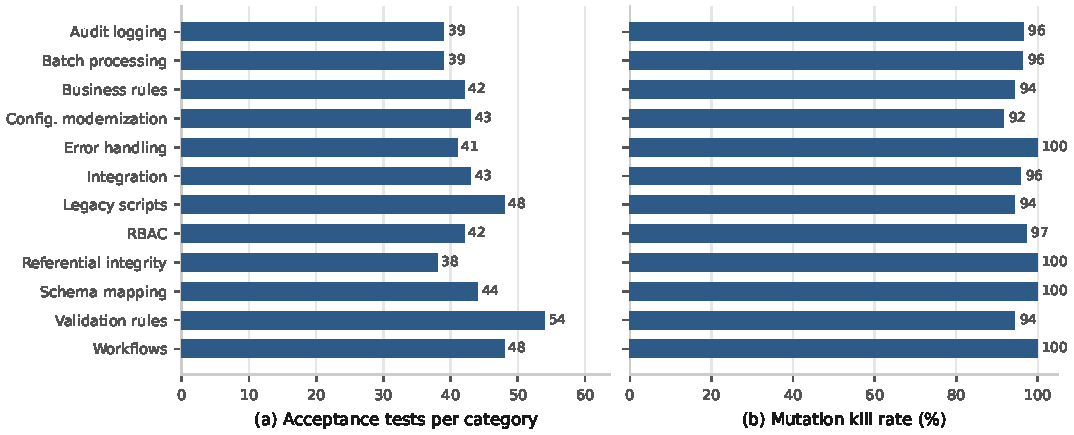
\includegraphics[width=\textwidth]{figures/F1_instrument_validation.pdf}
\caption{Instrument validation by category after the mutation-triage audit loop:
(a) acceptance tests per category; (b) mutation kill rate (remaining survivors are the
triaged equivalent/out-of-contract mutants). Generated by script from raw logs.}
\label{fig:val}
\end{figure*}

\begin{table}[t]
\caption{Instrument validation per category: reference pass, null-control pass, and mutation
kill rate (machine-generated from raw logs). Category rows are descriptive only (three cases
each); they support no between-category ranking.}
\label{tab:val}
\centering
\begin{tabular}{lccccc}
\toprule
Category & Ref. & Null & Mut. & Killed & Kill\% \\
\midrule
Audit logging & 39/39 & 0/39 & 28 & 27 & 96.4 \\
Batch processing & 39/39 & 0/39 & 27 & 26 & 96.3 \\
Business rules & 42/42 & 0/42 & 36 & 34 & 94.4 \\
Config.\ modernization & 43/43 & 0/43 & 12 & 11 & 91.7 \\
Error handling & 41/41 & 0/41 & 28 & 28 & 100.0 \\
Integration & 43/43 & 0/43 & 24 & 23 & 95.8 \\
Legacy scripts & 48/48 & 0/48 & 36 & 34 & 94.4 \\
RBAC & 42/42 & 0/42 & 36 & 35 & 97.2 \\
Referential integrity & 38/38 & 0/38 & 28 & 28 & 100.0 \\
Schema mapping & 44/44 & 0/44 & 36 & 36 & 100.0 \\
Validation rules & 54/54 & 0/54 & 36 & 34 & 94.4 \\
Workflows & 48/48 & 0/48 & 36 & 36 & 100.0 \\
\midrule
\textbf{Total} & \textbf{521/521} & \textbf{0/521} & \textbf{363} & \textbf{352} & \textbf{97.0} \\
\bottomrule

\end{tabular}
\end{table}

\begin{table}[t]
\caption{Model evaluation (executed): majority-collapsed case-level all-pass with Wilson
95\% CIs, repeated-trial reliability (pass\textasciicircum{}5, abbreviated p\textasciicircum{}5),
metered cost in USD for the full five-run cell, and mean per-call latency in seconds, per
condition (machine-generated from raw logs). For repaired C4 rows, latency reflects final
calls while cost sums all calls.}
\label{tab:models}
\centering
\begin{tabular}{llcccrr}
\toprule
Model & Cond. & Cases & 95\% CI & p\textasciicircum{}5 & \$ & s \\
\midrule
gpt-5.6-sol & C1 & 36/36 & [0.90, 1.00] & 1.000 & 4.53 & 14 \\
 & C2 & 36/36 & [0.90, 1.00] & 0.972 & 5.22 & 19 \\
 & C3 & 36/36 & [0.90, 1.00] & 1.000 & 5.96 & 16 \\
 & C4 & 36/36 & [0.90, 1.00] & 1.000 & 5.38 & 21 \\
\midrule
gpt-5.6-terra & C1 & 36/36 & [0.90, 1.00] & 0.972 & 2.38 & 9 \\
 & C2 & 35/36 & [0.86, 1.00] & 0.917 & 2.75 & 12 \\
 & C3 & 35/36 & [0.86, 1.00] & 0.917 & 3.04 & 14 \\
 & C4 & 36/36 & [0.90, 1.00] & 1.000 & 2.97 & 12 \\
\midrule
gpt-5.6-luna & C1 & 36/36 & [0.90, 1.00] & 0.917 & 0.27 & 10 \\
 & C2 & 34/36 & [0.82, 0.98] & 0.889 & 0.28 & 10 \\
 & C3 & 36/36 & [0.90, 1.00] & 0.917 & 0.33 & 14 \\
\bottomrule

\end{tabular}
\end{table}

\section{Ablation and Robustness Analysis}
\label{sec:ablation}
Condition ablations were run as planned; per the pre-committed analysis rule, every paired
condition contrast is reported with a bootstrap interval and flagged as underpowered (all
discordant counts are below the pre-registered threshold), so we describe directions without
significance claims. Two observations stand out. First, no condition \emph{helps}: every
non-zero case-level delta is zero or negative for the added-guidance conditions (C2/C3 vs.\
C1), and the checklist condition C2 produces the clearest cross-model \emph{regression}: the RBAC
equivalence case fails in at least one C2 run for all three models (majority-fails for the
mid and small tiers) while passing zero-shot in every run. Inspecting
the failing outputs shows the mechanism: C2's ``deny-by-default \ldots do not widen any permission'' instruction
pushes models to \emph{narrow} legacy grants (25 mismatched decisions in one frontier-model
output), which the bidirectional equivalence oracle rejects. Because every pre-registered contrast is underpowered, we report this as a reproducible
pattern with an inspectable mechanism rather than a hypothesis-tested causal effect; still,
guidance intended to protect security semantics coincided with their degradation --- a
caution for prompt-engineered migration pipelines.
Second, the repair condition C4 is the only intervention that changes outcomes, fixing all
observed failures within two redacted-feedback rounds at a 3--8\% cost overhead over C2. Run-to-run
robustness is quantified by pass\textasciicircum{}5 in Table~\ref{tab:models}; the
per-condition deltas with intervals are in the released \texttt{M2} table.

\section{Failure and Error Analysis}
\label{sec:failure}
Executed scope: the surviving-mutant triage described in Sec.~\ref{sec:results} was completed
for all 28 initial survivors, with every classification verified empirically (equivalence
argued and fuzz-checked; each claimed test gap reproduced by running the mutant, and each
added test shown to kill exactly its target mutant). The most instructive gaps were
security-relevant: one RBAC case never exercised the administrator-override branch, and one
schema-mapping case validated key sets but not mapped values, so migrations emitting empty
field values would have passed. These are precisely the failure modes the benchmark exists to
catch, which is why the audit loop is part of the released method rather than a one-off.
\textbf{Observed model-defect taxonomy (executed).} Reading every failing generation's
test-level output yields four defect classes, extending Pan et al.~\cite{pan2024lost} with
customization-specific failure modes: (1)~\emph{legacy-coercion defects} --- string values
preserved where the target requires numerics (the half-up rounding case fails on
\texttt{'10.5'} vs.\ \texttt{10.5}); (2)~\emph{completeness defects} --- a generated schema
silently drops a column, cascading into four referential-integrity test failures;
(3)~\emph{behavioral-logic defects} --- workflow close-lost transitions become no-ops when
the guard is mis-implemented; and (4)~\emph{access-decision non-equivalence} --- 25 decisions
diverging from the legacy matrix in a single output, in the \emph{narrowing} direction,
under checklist guidance (Sec.~\ref{sec:ablation}). Class~(4) is why the benchmark tests
decision \emph{equivalence} rather than one-sided ``no widening'': over-restriction is an
availability failure that a widening-only oracle would silently accept.

\section{Discussion}
\label{sec:discussion}
The pilot demonstrates that preservation-oriented, security-inclusive oracles for CRM
customization migration can be built with fully open provenance and validated without any
LLM in the evaluation path; the oracle-validity evidence (reference pass, null control,
mutation kill rate) is the load-bearing methodological claim~\cite{liu2023evalplus,
zhu2025rigorous}. The executed evaluation then delivers a calibration result the field needs:
with complete written specifications, the evaluated 2026 models migrate this customization
layer near-perfectly at the case level, and a third of the cases fall to a rule-based
transpiler with no model at all. What still fails --- and therefore where benchmarks and tooling should
focus --- is narrow and structural: idiosyncratic conventions (half-up rounding),
cross-artifact consistency, schema completeness, and access-control equivalence under
well-intentioned prompt guidance. Equally important for practice, single-shot case scores hid
the real differences between model tiers; repeated-trial reliability exposed them. Future
difficulty must come from withholding specification completeness (semantic archaeology), not
from more cases of the same shape.

\section{Practical Implications}
\label{sec:implications}
For practitioners, the case format doubles as a checklist of migration hazards: sentinel and
default conventions, collect-all validation semantics, ordered rule and transition evaluation,
scope-correct RBAC, privacy exclusions in outbound payloads, append-only audit with per-column
granularity, and configuration completeness. For tool builders, the harness provides an
integration target for migration pipelines. The executed evaluation adds two practical
lessons: prompt checklists meant to protect security semantics can backfire (the C2
regression), and single-shot spot checks understate model differences that repeated-trial
reliability exposes --- migration pipelines should gate on repeated runs, not single passes.

\section{Threats to Validity}
\label{sec:threats}
\textbf{Construct.} Acceptance tests approximate behavioral equivalence; mutation analysis
bounds but does not eliminate oracle weakness, and its coverage is itself bounded (Python
deliverables only; string-constant mutations dominate; the kill-rate interval treats mutants
as independent, which co-located mutants may violate). All remaining survivors are disclosed with their triage classifications. The
``modern platform'' target is a specification-defined Python/JSON interface rather than a
real vendor stack, which limits construct validity of the modernization dimension.
\textbf{Internal.} Reference solutions and tests were authored in the same project, partly
with the same generative-AI assistant that future evaluations may test; this creates both a
shared-blind-spot risk and an authoring-vendor circularity risk. Mitigations: the documented
semantics were frozen first, every expected value carries a written derivation, the
null-baseline and mutation-triage loops are executed and released, the evaluation slate must
include non-authoring-vendor models, and the artifact is public for adversarial scrutiny.
The risks are mitigated, not removed. \textbf{External.} Meridian CRM is synthetic and
simplified; results on it need not transfer to real vendor platforms, whose metadata formats
are more complex and less documented, and whose migrations involve re-deriving
\emph{undocumented} semantics --- here the semantics are documented, so tasks are closer to
specification-guided reimplementation than to semantic archaeology. Security claims are
single-tenant: cross-tenant isolation, a first-order concern in multi-tenant CRM platforms,
is out of scope. The evaluated slate is a single vendor's model family (a logged amendment
forced by credential availability); conclusions about ``current models'' generalize only to
that family, though the single-vendor slate also eliminates authoring-vendor circularity.
Near-ceiling case-level scores mean several contrasts rest on few discordant cases; all such
contrasts are interval-reported and flagged underpowered rather than tested to a verdict,
and the failure counts behind the defect taxonomy are small (31 of 1{,}620 generations).
Category-level conclusions rest on three cases each and are descriptive only. All executed
validation ran on a single environment (macOS/arm64, Python 3.14); an independent
reproduction is a release gate. \textbf{Contamination.} Artifacts are novel and
dated, but generic CRM conventions are widely represented in training corpora; post-release
training may contaminate future evaluations, and the release note says so.

\section{Ethics, Privacy, Licensing, and Data Governance}
\label{sec:ethics}
All artifacts are synthetic; no employer, customer, vendor, or personal data was used. Seed
records use fictional names from bundled word lists. Credentials appear only as vault
references; the benchmark tests that migrations keep it that way. Licenses: MIT (code),
CC~BY~4.0 (data/specifications). The audit-logging design also surfaces a real governance
tension the benchmark models but does not resolve: append-only audit trails retain old and
new field values, which real deployments must reconcile with data-subject erasure duties.
No human-subject research was conducted, and no human evaluation is claimed
(Sec.~\ref{sec:limitations}). Generative-AI assistance in constructing artifacts and drafting
text is disclosed in the Acknowledgments per IEEE policy.

\section{Reproducibility and Artifact Availability}
\label{sec:repro}
The artifact contains the legacy system and semantics specification, all cases with tests,
reference solutions and derivations, the harness, the mutation and aggregation tooling, raw
result logs with SHA-256 checksums, pinned dependencies, and a step-by-step non-destructive
reproduction guide (reproduced outputs are diffed against the archived logs rather than
overwriting them); every table in this paper is generated by script from raw logs.
[Repository/DOI placeholder: public hosting and archival deposit are pending; see Data
Availability.]

\section{Limitations}
\label{sec:limitations}
(1)~The evaluation covers one vendor's three model tiers under four conditions; other
vendors, agentic scaffolds beyond the bounded repair loop, and models postdating the runs are
out of scope, and near-ceiling case-level scores limit what the pilot can say about
between-model capability differences beyond reliability. (2)~Pilot scale (\NumCases{} cases, three per category) limits statistical power; category-level
analysis is descriptive. (3)~The legacy system is a documented simplification; enterprise
realism is bounded and vendor-specific formats are out of scope. Customization surfaces
deliberately excluded from the pilot include: role hierarchies and record-sharing rules beyond
role scopes, profile/permission-set models, leads and campaign management, record types and
layouts, approval processes, duplicate rules, multi-currency conversion, and dirty or
malformed legacy data (all fixtures and seed rows are clean, whereas real migrations are
dominated by data quality problems). (4)~No human-subject evaluation was conducted; nothing
is claimed about developer productivity, effort, or preference, and such claims would require
a separate, approved study. (5)~Reference solutions are released, so future models may train
on them; evaluations after the release date must address this, and held-out task variants
remain future work. (6)~The repair loop's redaction mechanism is leakage-audited (automated scan on every
feedback string, archived prompts), but absence of leakage cannot be proven. (7)~Workflow complexity is modest
relative to production CRM engines (no cross-object cascades or recursive triggers), so
workflow-hazard findings should be read as a lower bound on that dimension.

\section{Conclusion}
\label{sec:conclusion}
LegacyCRM-Bench operationalizes a question the benchmark landscape has not covered: whether
LLM-assisted migration preserves the configured behavior of enterprise CRM customizations,
security semantics included. The pilot contributes a documented synthetic legacy platform,
\NumCases{} cases with hand-derived executable oracles, a validated instrument, and a fully
executed, sandboxed, budget-capped evaluation of a deterministic baseline and three
commercial models. Its empirical message is double-edged: specification-complete
customization migration is nearly solved for the evaluated 2026 model tiers at the case
level, while
reliability, idiosyncratic legacy conventions, and access-control equivalence --- including a
checklist-associated regression --- remain the live failure surface. The benchmark's next
iteration should therefore withhold specification completeness and scale the quirk-bearing
case families; the released artifact is built to support exactly that extension.

\section*{Data Availability Statement}
Every artifact behind every reported number is synthetic and openly licensed: the fictional
Meridian CRM 4.2 specification and artifacts, the deterministic seed-data generator (fixed
seed; byte-identical regeneration), all \NumCases{} cases with acceptance tests, reference
solutions, and ground-truth derivations (CC~BY~4.0 for data and specifications, MIT for
code), the sandboxed harness and analysis scripts, the frozen prompts and protocol, and the
raw run logs with SHA-256 manifests --- including every model generation and the spend
ledger. No proprietary data, confidential information, internal system data, customer
records, or employer-owned data of any kind was used; no data originating from the author's
employer or from any commercial CRM deployment appears anywhere in this paper, and the
manuscript was prepared in compliance with standard employer confidentiality obligations.
The complete artifact will be released in a public GitHub repository with an archival DOI
upon acceptance [repository URL and DOI to be inserted at submission; release manifest
included in the artifact].

\section*{Acknowledgment (AI-Use Disclosure)}
Generative AI (Claude, Anthropic) was used, under the author's direction and review, to
assist in drafting manuscript text; designing and implementing the benchmark artifacts (the
synthetic Meridian CRM 4.2 specification, cases, acceptance tests, and reference solutions);
implementing the evaluation harness and analysis scripts; and compiling the literature
search. All benchmark semantics and verification results were validated by executable tests
and all references were verified against primary sources. All research direction,
experimental design decisions, and conclusions are the author's own work and were reviewed
and approved by the author, who takes full responsibility for all content.

\bibliographystyle{IEEEtran}
\bibliography{refs}

\begin{IEEEbiographynophoto}{Chitrapradha Ganesan}
(Senior Member, IEEE) received the M.Eng.\ degree in Software Engineering from Anna
University, Chennai, India. She has over 19 years of experience in enterprise software
engineering, with specialization in CRM architecture, AI-driven automation, data
integration, and retrieval-augmented generation systems. Her research interests include
enterprise AI, knowledge-grounded generation, CRM decision support, hybrid retrieval, and
responsible AI systems.
\end{IEEEbiographynophoto}

\end{document}
